5. По теореме Виета $x_1+x_2=15,\ x_1x_2=q.$ Тогда $\cfrac{1}{x_1}+\cfrac{1}{x_2}=\cfrac{x_1+x_2}{x_1x_2}=\cfrac{15}{q}=\cfrac{5}{12}\Rightarrow q=36.$ Построим параболу $x^2-15x+36$ по трём точкам $(4;0),\ (12;0),\ \left(\cfrac{15}{2}, -\cfrac{81}{4}
ight).$
$$ 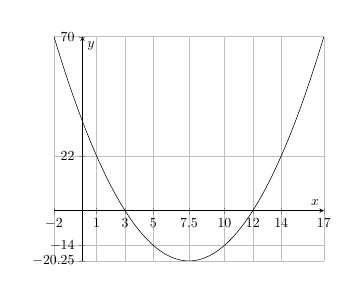
\begin{tikzpicture}[scale=0.5]
\begin{axis}[
    axis lines = middle,
    grid=major,
    legend pos={south west},
    xlabel = {$x$},
    ylabel = {$y$},
    %ymin=-80,
    %ymax=250,
    xtick={-2, 1, 3, 5, 7.5, 10, 12, 14, 17},
    ytick={70,22,-14,-20.25,-30}          ]
	\addplot[domain=-2:17, samples=100, color=black] {x*x-15*x+36};
%\addplot[domain=-3.1:2.5, samples=100, color=red] {70*abs(1-2*abs(abs(x)-2))-10*x^2+10*x-70};
	%\addlegendentry{$\text{Рис. 1}$};
\end{axis}
\end{tikzpicture}$$
